\documentclass{beamer}

% Use Metropolis theme
\usetheme{metropolis}

% Packages
\usepackage{graphicx}
\usepackage{booktabs}
\usepackage{amsmath}
\usepackage{amssymb}
\usepackage{bbm}

% Title information
\title{Employee Ownership Support Programs and ESOP Participation}
\subtitle{Evidence from Colorado's HB17-1214}
\author{Mitchell Ballif \and Patrick Beal \and Will Cheney \and Soren Pack}
\date{\today}
\institute{}

\begin{document}

% Slide 1: Title
\begin{frame}
\titlepage
\end{frame}

% Slide 2: Research Question and Motivation
\begin{frame}{Research Question}
\LARGE
\textbf{Did Colorado's policy increase ESOP adoption?}

\vspace{2em}
\large

\textbf{Why does this matter?}

\begin{itemize}
    \item ESOPs increase wealth for workers who own company shares
    \item Small businesses struggle with high transition costs
    \item Colorado offered education and financing in 2017
    \item Can this approach increase ESOP adoption?
\end{itemize}

\end{frame}

% Slide 3: Empirical Strategy
\begin{frame}{Empirical Strategy}

\large
\textbf{Compare Colorado to Utah before and after 2017}



\begin{itemize}
    \item Treatment: Colorado firms after 2017
    \item Control: Utah firms (similar economy, no policy)
    \item Data: 2012--2025 5500 Form pension filings
    \item State and year fixed effects
    \item Standard errors clustered at firm level
\end{itemize}

\[
Y_{it} = \delta (\text{Colorado}_i \times \text{Post}_t) + \lambda_i + \mu_t + \epsilon_{it}
\]



Where:
\begin{itemize}
    \footnotesize
    \item $Y_{it}$: Outcome (ESOP firms, participants, assets)
    \item $\text{Colorado}_i \times \text{Post}_t$: Treatment indicator
    \item $\delta$: DiD estimator (treatment effect)
    \item $\lambda_i$: State fixed effects
    \item $\mu_t$: Year fixed effects
\end{itemize}

\vspace{0.5em}
\normalsize
Key assumption: Both states had similar trends before 2017

\end{frame}

% Slide 4: Identifying Assumptions - Event Study
\begin{frame}{Testing Parallel Trends}

\centering
\begin{minipage}{0.48\textwidth}
    \centering
    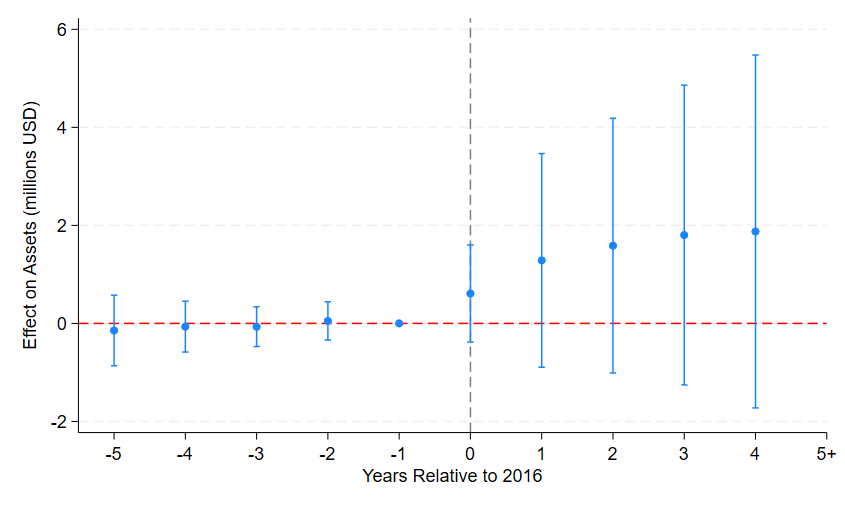
\includegraphics[width=\textwidth]{./images/data_portion/firm_event_assets_state_FE.png}
    \vspace{-1.5em}

    {\tiny Total ESOP Assets}
\end{minipage}
\hfill
\begin{minipage}{0.48\textwidth}
    \centering
    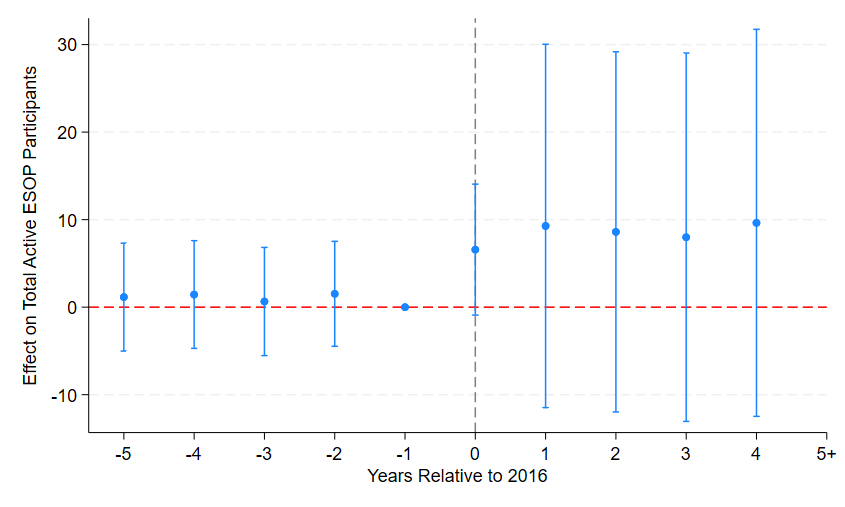
\includegraphics[width=\textwidth]{./images/data_portion/firm_event_act_partcp_state_FE.png}
    \vspace{-1.5em}

    {\tiny Total ESOP Participants}
\end{minipage}

\vspace{0.5em}
\large

\begin{itemize}
    \item Before 2017: Colorado and Utah followed same trend
    \item \alert{Parallel trends assumption holds in the pre-trend}
\end{itemize}

\end{frame}

% Slide 5: Identifying Assumptions - Validity
\begin{frame}{Are Our Assumptions Valid?}

\normalsize

\begin{itemize}
    \item[\textcolor{green!60!black}{$\checkmark$}] \textbf{Compliance:} Treatment only in Colorado
    \begin{itemize}
        \footnotesize
        \item HB17-1214 enacted exclusively in Colorado
        \item Utah had no access to programs, no comparable policies
    \end{itemize}

    \vspace{1em}

    \item[\textcolor{green!60!black}{$\checkmark$}] \textbf{Parallel Trends:} Same trends before 2017
    \begin{itemize}
        \footnotesize
        \item Event study shows pre-treatment coefficients $\approx 0$
    \end{itemize}

    \vspace{1em}

    \item[\textcolor{green!60!black}{$\checkmark$}] \textbf{SUTVA:} No spillovers to Utah
    \begin{itemize}
        \footnotesize
        \item Benefits require Colorado presence
        \item ESOP transitions costly, unlikely cross-state influence
    \end{itemize}

    \vspace{1em}

    \item[\textcolor{green!60!black}{$\checkmark$}] \textbf{Exclusion Restriction:} Policy affects outcome only through ESOP adoption
    \begin{itemize}
        \footnotesize
        \item HB17-1214 specifically targets ESOP formation
        \item Education + loans directly reduce ESOP transition costs
        \item Small budget (\$200k/year), no broader economic impacts
        \item Policy doesn't affect firms through other channels
    \end{itemize}
\end{itemize}

\end{frame}

% Slide 6: Main Results - DiD Table
\begin{frame}{Main Results}

\begin{table}
\centering
\begin{tabular}{lcc}
\toprule
\textbf{Outcome} & \textbf{Effect} & \textbf{SE} \\
\midrule
ESOP Firms & 0.006 & (0.005) \\
Total Participants & 25.2 & (17.4) \\
Total Assets (\$) & 2.88M* & (1.61M) \\
Active Participants & 22.3 & (15.4) \\
\bottomrule
\end{tabular}
\end{table}

\vspace{1em}
\LARGE

\alert{The policy had no significant effect}

\vspace{.5em}
\large
\begin{itemize}
    \item Almost all results statistically insignificant
    \item Effects are economically small
\end{itemize}

\vspace{.5em}

\normalsize
\textbf{\alert{MAJOR CAVEAT:}} Only 2 states $\Rightarrow$ cannot cluster at state level \\
Standard errors \alert{ understated}, precision \alert{overstated}

\end{frame}

% Slide 7: Robustness - Synthetic Control
\begin{frame}{Robustness: Synthetic Control}

\centering
\begin{minipage}{0.48\textwidth}
    \centering
    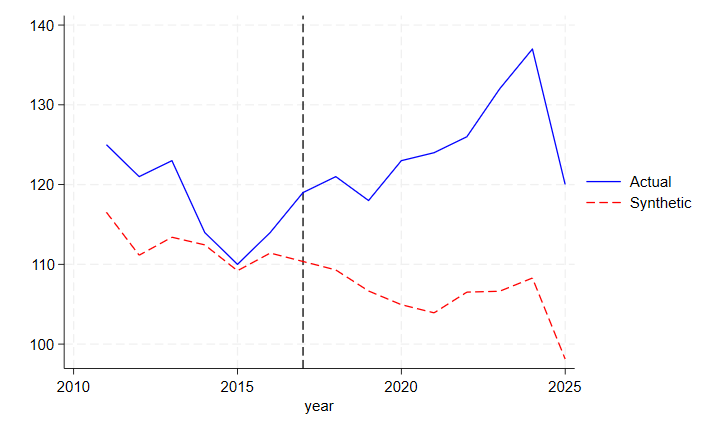
\includegraphics[width=\textwidth]{./images/esop_firms_num_synth.png}
    \vspace{-1.5em}

    {\tiny Number of ESOP Firms}
\end{minipage}
\hfill
\begin{minipage}{0.48\textwidth}
    \centering
    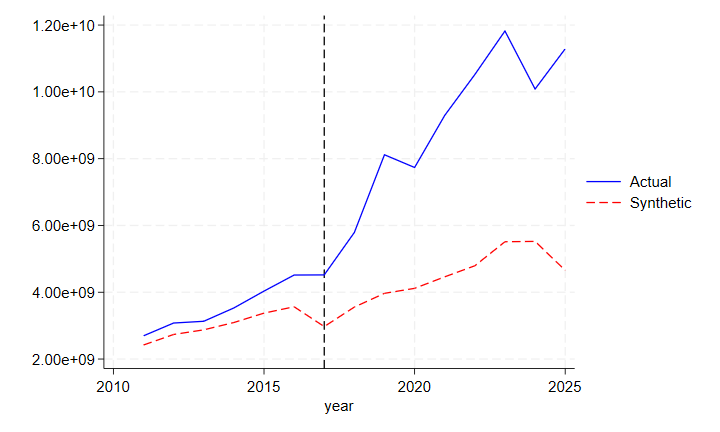
\includegraphics[width=\textwidth]{./images/esop_tot_assets_boy_amt_synth.png}
    \vspace{-1.5em}

    {\tiny Total ESOP Assets}
\end{minipage}

\vspace{0.5em}
\large

\begin{itemize}
    \item Synthetic control uses all US states as comparison
    \item Shows larger effects than our main analysis
    \item \alert{Problem:} Poor fit before 2017 means results not reliable
    \item We trust our main DiD estimates more
\end{itemize}

\end{frame}

% Appendix
\appendix

\begin{frame}{Appendix: Full Regression Results}

\begin{table}
\centering
\caption*{Table 1: Difference-in-Differences Results (Year and State Fixed Effects)}
\tiny
\begin{tabular}{lccccc}
\toprule
Variable & (1) ESOP Firm & (2) Total Partcps. & (3) Total Assets & (4) Active Partcps. & (5) Partcp. Rate \\
\midrule
\textbf{DiD} & 0.00607 & 25.19 & 2,878,102.7* & 22.29 & 0.00613 \\
             & (0.00486) & (17.35) & (1,611,044.2) & (15.37) & (0.00426) \\
\textbf{Constant} & 0.0215*** & 18.16*** & 1,258,818.5*** & 13.99*** & 0.0175*** \\
                  & (0.00131) & (6.636) & (445,403.5) & (5.124) & (0.00113) \\
\midrule
\textbf{Observations} & 209,399 & 209,399 & 209,399 & 209,399 & 191,912 \\
\bottomrule
\end{tabular}
\end{table}

\vspace{0.5em}
\scriptsize
Standard errors (clustered at firm level) in parentheses. * $p<0.10$, ** $p<0.05$, *** $p<0.01$ \\
\vspace{0.3em}
\textit{Note:} Standard errors are clustered at the firm level. Theoretically appropriate state-level clustering is infeasible with only two states.

\end{frame}

\end{document}
